\newpage
\section{OpenMLE-Gym Details}

\subsection{Task Construction and Selection}
\label{app:data-construction}

This appendix details the construction, validation, and selection mechanisms summarized in Section~\ref{sec:task-curation-data-construction}. All three task sources follow the shared executable contract defined there; we focus below on the automated competition branch and its post-construction gates.

\textbf{Competition-construction state machine.}
The builder consumes the candidate slugs remaining after upstream filtering. Independent competitions can be dispatched concurrently, while each competition follows an ordered state machine so that downstream stages run only after their prerequisites succeed.

For each slug, the pipeline downloads and recursively unpacks the competition archive, preserves the source assets, and retrieves the pre-computed competition overview and dataset description. A tool-assisted file-perception stage then enumerates the local tree, probes tabular files for structural summaries and sampled rows, and reads textual documentation. The resulting inventory and competition metadata jointly ground the generated task description, avoiding reliance on either web metadata or filenames alone.

\textbf{Executable construction and validation.}
Conditioned on the generated description, the pipeline produces and executes \texttt{prepare.py} to create deterministic train/test splits, copy associated modality files, expose participant-visible inputs, and isolate held-out answers. Execution success alone is insufficient: the builder checks for the task description, training data, test inputs, sample submission, and private test answers before accepting the package. A failed attempt clears its partial processed outputs and returns the execution error to the next generation attempt, preventing malformed intermediate state from being reused.

After preparation succeeds, the pipeline generates the task-specific \texttt{metric.py} from the task description together with samples of the submission and private-answer schemas. Metric generation and metric validation are separate stages. The latter dynamically loads the generated evaluator and scores \path{data/public/sample_submission.csv} against \path{data/private/test_answer.csv}; import errors, execution errors, missing inputs, or a missing score fail this gate before semantic assessment.

Raw assets may remain in \texttt{raw/}. For storage-reduced packages, the generated file inventory is first preserved as \texttt{raw.txt} before the raw directory is removed. The quality record consumes this inventory when available; otherwise, raw-data use is assessed from the presence of source assets, \texttt{prepare.py}, and the resulting public/private data.

\begin{figure*}[t]
  \centering
  \includegraphics[page=3,width=\textwidth]{figures/task-curation.pdf}
  \caption{Automated competition task construction. Competition metadata and local-file evidence ground package generation; execution feedback revises failed preparation before metric validation and semantic gating.}
  \label{fig:competition-task-construction}
\end{figure*}

\textbf{Metadata profiling and semantic quality assessment.}
Post-construction profiling annotates modality and task type from the task description, measures raw and processed data size, classifies the expected CPU/GPU requirement, and records metric-validation output. These stages can process task chunks concurrently but restore the original task order when writing the aggregate metadata.

The quality evaluator first inspects package structure and executes the metric smoke test. Missing critical files or failed metric execution deterministically yield \texttt{not\_recommended}. For packages that pass these hard gates, the semantic judge receives the description, \texttt{prepare.py}, train/test sizes, processed-data size, auxiliary file types, sampled public and held-out rows, available raw inventory, and metric result. It returns scores for task validity, data sufficiency, raw-data usage, task complexity, and data quality, together with one of \texttt{recommended}, \texttt{conditional}, or \texttt{not\_recommended}. The evaluator records these judgments without mutating the package collection; final aggregation admits only metric-valid tasks with the strict \texttt{recommended} decision.

\textbf{Metadata accounting.}
The distribution plots in Figure~\ref{fig:task-scale-distribution} use mutually exclusive normalized groups. Tasks containing multiple modalities are assigned to Multimodal, compound task labels to Multitask, and rare labels to Other. Package size is measured from constructed task contents.






\subsection{OpenMLE-Gym Execution Infrastructure}
\label{app:sandbox}

\textbf{Architecture.}
Figure~\ref{fig:sandbox-architecture} expands the execution backend summarized in Section~\ref{sec:gym-sandbox-execution}, exposing the API boundary and the separation among scheduling, isolated workers, shared job state, and returned feedback.

\begin{figure}[h!]
  \centering
  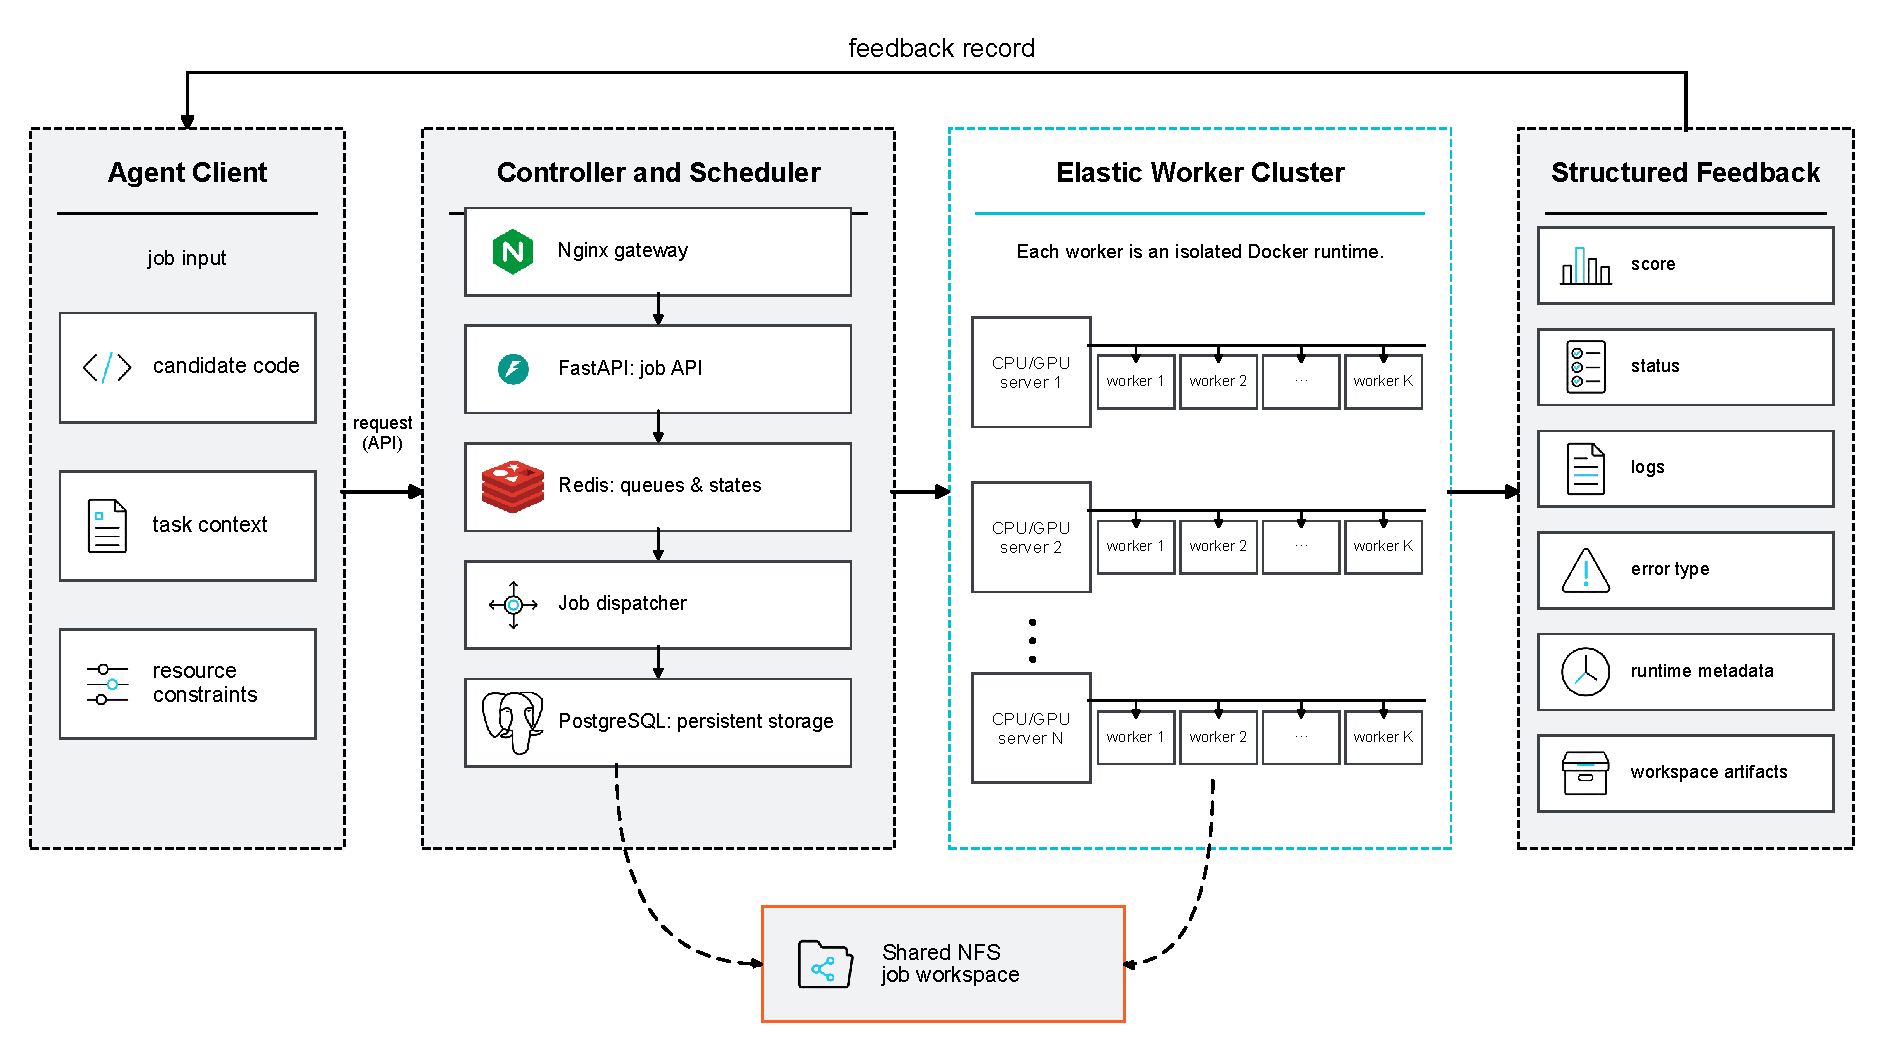
\includegraphics[width=\linewidth]{figures/sandbox_architecture}
  \caption{OpenMLE-Gym execution-backend architecture. Agent requests are dispatched to CPU/GPU Docker workers, which execute candidate programs against task data and evaluators and return structured feedback.}
  \label{fig:sandbox-architecture}
\end{figure}

\textbf{Representative feedback cases.}

Table~\ref{tab:sandbox-real-cases} grounds the six feedback modes summarized in Section~\ref{sec:gym-sandbox-execution} with representative jobs. Each row connects a concrete trigger to returned fields and their usable signal; the following transcript traces one failure end to end.

\begin{table}[h!]
  \centering
  \caption{Representative coverage of sandbox feedback modes from real job logs. Each row abstracts one real job into its trigger, returned feedback fields, and usable signal for training or evaluation.}
  \label{tab:sandbox-real-cases}
  \vspace{0.4em}
  \footnotesize
  \setlength{\tabcolsep}{5pt}
  \renewcommand{\arraystretch}{1.14}
  \begin{tabular}{@{}>{\raggedright\arraybackslash}p{0.19\linewidth}>{\raggedright\arraybackslash}p{0.73\linewidth}@{}}
    \toprule
    \textbf{Case} & \textbf{Trigger, feedback, and usable signal} \\
    \midrule
    \textbf{Success}
    & \textbf{Trigger:} candidate finishes training and writes \texttt{submission.csv}.\newline
      \textbf{Feedback:} \texttt{completed}; score $0.9991$; logs; runtime metadata; validated artifact.\newline
      \textbf{Signal:} valid scored trajectory. \\
    \addlinespace[2pt]
    \textbf{Runtime error}
    & \textbf{Trigger:} code calls an unsupported PyTorch API argument.\newline
      \textbf{Feedback:} \texttt{code\_execution\_error}; null score; exit code; traceback.\newline
      \textbf{Signal:} executable code defect before scoring. \\
    \addlinespace[2pt]
    \textbf{Missing code}
    & \textbf{Trigger:} submitted \texttt{main.py} is empty.\newline
      \textbf{Feedback:} \texttt{code\_missing}; null score; immediate pre-execution diagnostic.\newline
      \textbf{Signal:} invalid request filtered before worker execution. \\
    \addlinespace[2pt]
    \textbf{Missing submission}
    & \textbf{Trigger:} process exits successfully but does not write \texttt{submission.csv}.\newline
      \textbf{Feedback:} \texttt{submission\_missing}; null score; missing-artifact log.\newline
      \textbf{Signal:} distinguishes process success from valid submission. \\
    \addlinespace[2pt]
    \textbf{Scoring failed}
    & \textbf{Trigger:} submitted file violates the evaluator schema.\newline
      \textbf{Feedback:} \texttt{scoring\_failed}; null score; evaluator-side validation error.\newline
      \textbf{Signal:} invalid artifact separated from low task performance. \\
    \addlinespace[2pt]
    \textbf{Timeout}
    & \textbf{Trigger:} long-running training exceeds the execution budget.\newline
      \textbf{Feedback:} \texttt{timeout}; null score; timeout metadata; partial stdout.\newline
      \textbf{Signal:} resource or algorithmic inefficiency with retained debugging evidence. \\
    \bottomrule
  \end{tabular}
\end{table}

\textbf{End-to-end transcript.}

The following transcript traces a failed GPU job from the submitted program through execution, the structured result, and the diagnostic traceback needed to repair it.

\noindent\textbf{Step 1: Agent request.}
The agent submits a generated Python program together with the task data directory and resource constraints.
In this job, the task is brain-tumor MRI classification and the public data directory is exposed to the program through \texttt{DATA\_DIR}.

\begin{SandboxTranscript}
name: brain-tumor-detection-mri@1
code: <candidate Python program>
data_dir: <task-public-data-dir>
resource_type: gpu
gpu_count: 1
timeout: 3600
\end{SandboxTranscript}

The server materializes the submitted code as \texttt{main.py} inside the job workspace.
The excerpt below shows the part that later triggers the runtime error; unrelated dataset loading, model definition, and training code is omitted.

\begin{SandboxTranscript}
# Initialize model
device = torch.device("cuda" if torch.cuda.is_available() else "cpu")
model = BrainTumorClassifier(
    model_name="efficientnet_b0",
    pretrained=True,
    dropout=0.3,
).to(device)

# Loss function with label smoothing
criterion = nn.BCEWithLogitsLoss(label_smoothing=0.1)

optimizer = optim.AdamW(model.parameters(), lr=1e-4, weight_decay=1e-4)
...
\end{SandboxTranscript}

\noindent\textbf{Step 2: Sandbox execution.}
The control server materializes the job workspace, assigns an idle GPU worker, and runs the candidate inside an isolated Docker worker.
The actual command binds the task data path into the process environment, captures stdout/stderr into the job workspace, and preserves the process exit code.

\begin{SandboxTranscript}
export DATA_DIR=<task-public-data-dir>
python <sandbox-job-workspace>/code/main.py
2>&1 | tee -a <sandbox-job-workspace>/sandbox_stdout.log
\end{SandboxTranscript}

\noindent\textbf{Step 3: Sandbox feedback.}
The returned record preserves machine-readable status, runtime, and artifact fields alongside the human-readable log. Because the program fails during execution, the evaluator is not invoked and the score remains null.

\begin{SandboxTranscript}
job_id: job_<id>
score: null
status: failed
logs:
  stdout_stderr: <sandbox-job-workspace>/sandbox_stdout.log
  diagnostic_excerpt: TypeError in BCEWithLogitsLoss(...)
error_type: code_execution_error
runtime_metadata:
  resource_type: gpu
  exit_code: 1
  shell_runtime: 11.88s
  evaluation: skipped because code execution failed
workspace_artifacts:
  workspace: <sandbox-job-workspace>
  submission: missing
  preserved_files: code/main.py, sandbox_stdout.log
\end{SandboxTranscript}

\noindent\textbf{Step 4: Diagnostic log.}
The key diagnostic is the traceback, which points directly to the generated line that is incompatible with the installed PyTorch API.

\begin{SandboxTranscript}
Traceback (most recent call last):
  File "<sandbox-job-workspace>/code/main.py", line 151, in <module>
    criterion = nn.BCEWithLogitsLoss(label_smoothing=0.1)
TypeError: BCEWithLogitsLoss.__init__() got an unexpected keyword argument
  'label_smoothing'
\end{SandboxTranscript}

Together, the status, error, runtime, artifact, and traceback fields localize the failure before evaluation and provide concrete evidence for the next repair action.

\section{OpenMLE-ERL Details}
\label{app:training-configs}

\subsection{SFT Data Generation}
\label{app:sft-warm-start}

\textbf{Parallel Path Sampling.}
The teachers first generate multiple independent \textsc{Draft} solutions for each standardized task, and every candidate is executed in the corresponding task sandbox. The first collection batch uses GLM-4.7. Among candidates with valid execution scores for the same task, we remove solutions with duplicate scores, rank the remaining candidates by score, and retain at most the Top-4. The released corpus contains 11,519 examples from this batch. The second batch uses both GLM-4.7 and Qwen3-30B-A3B-Thinking-2507. After execution and output-length screening, candidates from both teachers are jointly ranked within each task: a GLM-4.7 candidate is retained when it falls in the joint Top-4, whereas a Qwen candidate is retained only when it ranks first overall. Consequently, each task still contributes at most four examples rather than four GLM candidates plus an additional Qwen candidate. After corpus-level assembly, the released corpus contains 5,726 examples from this batch, comprising 5,075 GLM-4.7 and 651 Qwen examples. The two batches contribute 17,245 full-response examples in total.

\textbf{Evolutionary Path Sampling.}
Complete solutions expose final programs but do not directly supervise how execution feedback should be used to revise an existing solution. We therefore use GLM-4.7 to drive AIRA-Evo searches with \textsc{Draft}, \textsc{Improve}, \textsc{Crossover}, and \textsc{Debug}, producing search trees with parent relations, program versions, execution feedback, and task scores. A local segment begins at a \textsc{Draft}, \textsc{Improve}, or \textsc{Crossover} node and follows its consecutive \textsc{Debug} descendants along true parent--child edges; the segment ends when a branch reaches another \textsc{Draft}, \textsc{Improve}, or \textsc{Crossover} node. A \textsc{Draft} segment must end with a positive score, an \textsc{Improve} segment must outperform its parent program, and a \textsc{Crossover} segment must outperform the better of its two parents. Retained endpoints must additionally attain a bronze, silver, or gold level.

Single-step segments whose roots are themselves medal-level endpoints are retained directly. For multi-step segments, DeepSeek-V4-Pro reads each complete segment---including the task constraints, parent code, endpoint code, adjacent code changes, and stepwise execution feedback---and determines whether the strategy, program structure, or error repair introduced by each step is inherited by later steps and contributes to the final effective solution. After corpus-level assembly, the evolutionary path contributes 9,014 trajectory-step examples to the released corpus.

\textbf{Assembly and final corpus distribution.}
We normalize complete solutions and trajectory steps into the same system--user--assistant message structure and perform exact deduplication over the normalized full \texttt{messages} content. We then apply the target model's chat template to the full message sequence and exclude examples longer than 32,768 tokens. The released SFT corpus contains 26,259 training examples.

Of the released corpus, 17,245 full responses account for 65.7\%, and 9,014 trajectory steps account for 34.3\%. At the atomic-operator level, \textsc{Draft}, \textsc{Improve}, \textsc{Crossover}, and \textsc{Debug} contribute 19,436, 1,741, 742, and 4,340 examples, respectively, corresponding to 74.0\%, 6.6\%, 2.8\%, and 16.5\%. The median full-message lengths are 8,407 tokens for full responses and 14,051 tokens for trajectory steps; the latter are longer because they include parent programs, execution feedback, and local search context.

\begin{figure}[t]
  \centering
  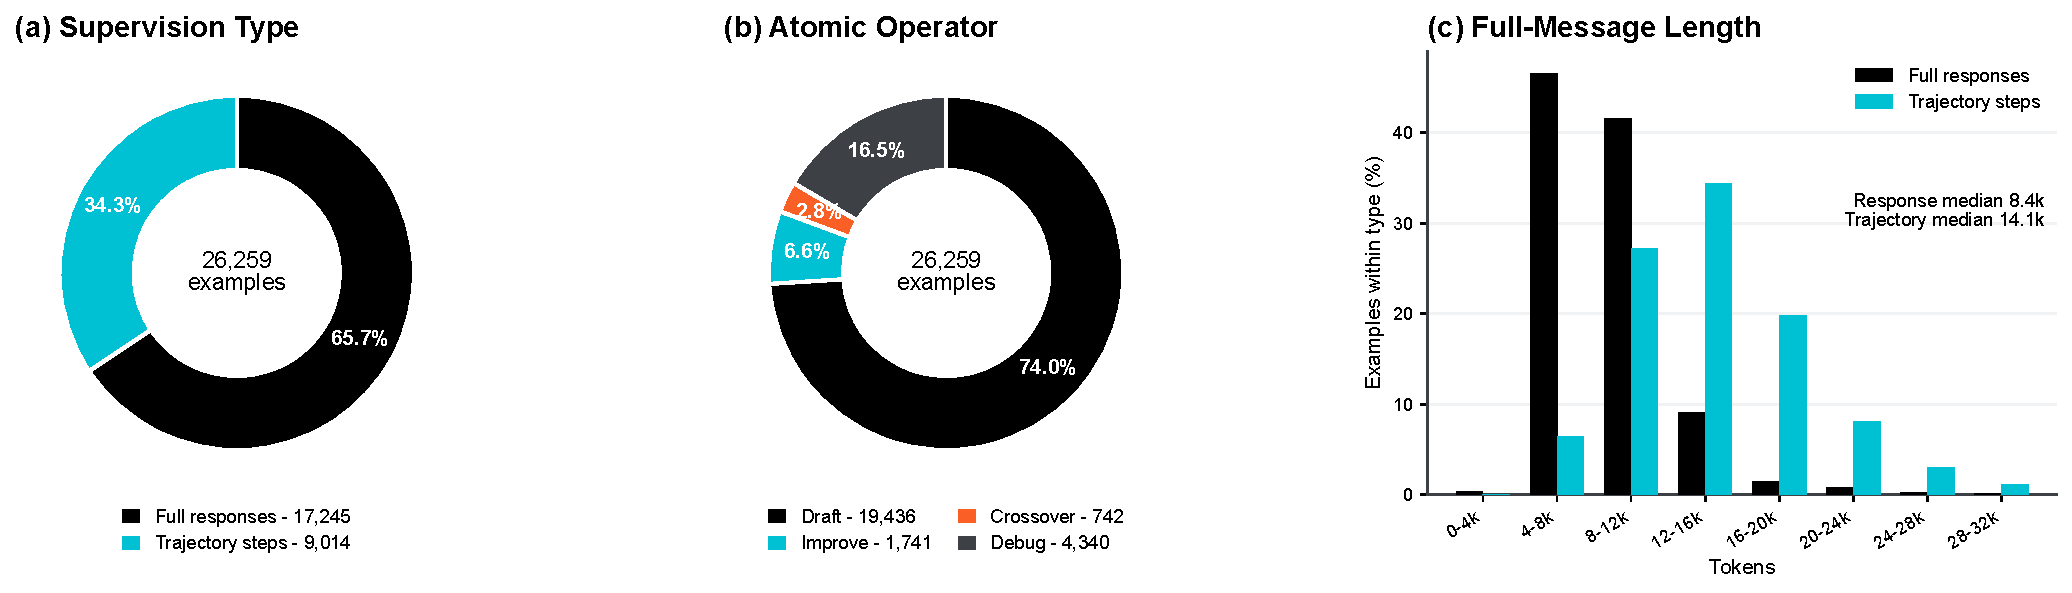
\includegraphics[width=\linewidth]{figures/final_sft_data_distribution.pdf}
  \caption{Distribution of the final SFT corpus. (a) Relative proportions of full-response and trajectory-step supervision among the 26,259 training examples. (b) Distribution of the four atomic operators. (c) Full-message length distributions for the two supervision types; each bar reports the percentage within its corresponding supervision type.}
  \label{fig:sft-final-data-distribution}
\end{figure}

\textbf{Prompt for trajectory-step selection.}
The annotator follows a causal-inheritance criterion: a step is retained only when its core strategy, necessary intermediate state, or critical error repair is inherited by later steps and makes a concrete contribution to the segment endpoint. Cosmetic edits, blind retries, changes that merely reduce training scale to avoid resource limits, and failed environment modifications or external-network accesses are discarded. We use DeepSeek-V4-Pro with temperature 0 and a maximum output length of 4,096 tokens, requiring a fixed JSON schema that accounts for every input step. The production system prompt is reproduced below.

\VerbatimInput[
  fontsize=\scriptsize,
  frame=single,
  framesep=1.5mm,
  framerule=0.3pt,
  rulecolor=\color{black!35},
  breaklines=true,
  breakanywhere=true,
  breaksymbolleft={}
]{sections/prompts/trajectory_step_selection_system_prompt.txt}

Each request instantiates the following input template. \texttt{PARENT\_CODES} is omitted for \textsc{Draft}, contains one parent for \textsc{Improve}, and contains two parents for \textsc{Crossover}.

\begin{SandboxTranscript}
Annotate the following candidate trajectory using system instructions.

<TASK_SYSTEM_PROMPT>
{original task environment and constraints}
</TASK_SYSTEM_PROMPT>

<TASK_USER_PROMPT>
{original task description}
</TASK_USER_PROMPT>

<PARENT_CODES>
{one parent for Improve; two parents for Crossover; omitted for Draft}
</PARENT_CODES>

<FINAL_SOLUTION_CODE>
{complete endpoint code}
</FINAL_SOLUTION_CODE>

<TRAJECTORY_STEPS>
{root full code, subsequent full-file diffs, and execution feedback}
</TRAJECTORY_STEPS>
\end{SandboxTranscript}


\subsection{SFT Training Configuration}

Table~\ref{tab:sft-warm-start-config} summarizes the core training settings used for the executable SFT warm starts of \thirtybmodel{} and \thirtyfivebmodel{}.

\begin{table}[h!]
\centering
\caption{Core SFT hyperparameters for \thirtybmodel{} and \thirtyfivebmodel{}. Settings shared by both models are centered across the two model columns.}
\label{tab:sft-warm-start-config}
\vspace{0.4em}
\footnotesize
\setlength{\tabcolsep}{3.5pt}
\renewcommand{\arraystretch}{1.08}
\begin{tabular}{@{}>{\raggedright\arraybackslash}p{0.18\linewidth}>{\raggedright\arraybackslash}p{0.37\linewidth}>{\raggedright\arraybackslash}p{0.37\linewidth}@{}}
\toprule
Item & \thirtybmodel{} & \thirtyfivebmodel{} \\
\midrule
Base model & Qwen3-30B-A3B-Thinking-2507 & Qwen3.6-35B-A3B \\
\addlinespace[3pt]
Training stage & \multicolumn{2}{>{\centering\arraybackslash}p{0.76\linewidth}}{Full-parameter SFT} \\
\addlinespace[3pt]
Training framework & \multicolumn{2}{>{\centering\arraybackslash}p{0.76\linewidth}}{SLIME with Ray and Megatron-LM} \\
\addlinespace[3pt]
\addlinespace[3pt]
Template / thinking mode & \texttt{qwen3} loss mask; \texttt{<think>} supervision retained & \texttt{qwen3\_5}-compatible loss mask; \texttt{<think>} supervision retained \\
\addlinespace[3pt]
Context cutoff & \multicolumn{2}{>{\centering\arraybackslash}p{0.76\linewidth}}{32,768 tokens} \\
\addlinespace[3pt]
Precision & \multicolumn{2}{>{\centering\arraybackslash}p{0.76\linewidth}}{bfloat16} \\
\addlinespace[3pt]
Global batch size & \multicolumn{2}{>{\centering\arraybackslash}p{0.76\linewidth}}{128} \\
\addlinespace[3pt]
Per-device batch size & \multicolumn{2}{>{\centering\arraybackslash}p{0.76\linewidth}}{1 with dynamic batching} \\
\addlinespace[3pt]
Gradient accumulation & 64 microbatches per update & 32 microbatches per update \\
\addlinespace[3pt]
Learning rate & \multicolumn{2}{>{\centering\arraybackslash}p{0.76\linewidth}}{$3.0\times10^{-5}$} \\
\addlinespace[3pt]
Scheduler / warmup & \multicolumn{2}{>{\centering\arraybackslash}p{0.76\linewidth}}{cosine decay to 0, 0.1 warmup fraction} \\
\addlinespace[3pt]
Epochs & \multicolumn{2}{>{\centering\arraybackslash}p{0.76\linewidth}}{3} \\
\bottomrule
\end{tabular}
\end{table}

\Needspace{0.58\textheight}
\subsection{RL Training Configuration}

Table~\ref{tab:rl-training-config} summarizes the verified RL settings for \thirtybmodel{} and \thirtyfivebmodel{} while retaining the original configuration fields.

\begin{table}[h!]
\centering
\caption{RL hyperparameters for \thirtybmodel{} and \thirtyfivebmodel{}. Settings shared by both models are centered across the two model columns.}
\label{tab:rl-training-config}
\vspace{0.4em}
\footnotesize
\setlength{\tabcolsep}{3.2pt}
\renewcommand{\arraystretch}{1.06}
\begin{tabular}{@{}>{\raggedright\arraybackslash}p{0.18\linewidth}>{\raggedright\arraybackslash}p{0.37\linewidth}>{\raggedright\arraybackslash}p{0.37\linewidth}@{}}
\toprule
Item & \thirtybmodel{} & \thirtyfivebmodel{} \\
\midrule
RL initialization & SFT warm-start checkpoint trained from Qwen3-30B-A3B-Thinking-2507 & SFT warm-start checkpoint trained from Qwen3.6-35B-A3B \\
\addlinespace[3pt]
Training framework & \multicolumn{2}{>{\centering\arraybackslash}p{0.76\linewidth}}{SLIME with Ray and SGLang} \\
\addlinespace[3pt]
\addlinespace[3pt]
Operator sampling probability & \multicolumn{2}{>{\centering\arraybackslash}p{0.76\linewidth}}{\textsc{Draft} 0.50, \textsc{Improve} 0.17, \textsc{Debug} 0.17, \textsc{Crossover} 0.16} \\
\addlinespace[3pt]
Rollout group & \multicolumn{2}{>{\centering\arraybackslash}p{0.76\linewidth}}{16 prompts per rollout, 16 samples per prompt, global batch size 128, 2 optimizer steps per rollout} \\
\addlinespace[3pt]
Generation & \multicolumn{2}{>{\centering\arraybackslash}p{0.76\linewidth}}{temperature 1.0, maximum response length 24,576 tokens} \\
\addlinespace[3pt]
\addlinespace[3pt]
Advantage / objective & \multicolumn{2}{>{\centering\arraybackslash}p{0.76\linewidth}}{GSPO with TTT-Discover-style reward post-processing, clip $\epsilon=3.5\times10^{-4}$, TIS enabled} \\
\addlinespace[3pt]
Optimizer & \multicolumn{2}{>{\centering\arraybackslash}p{0.76\linewidth}}{Adam, learning rate $1.0\times10^{-6}$, constant schedule, weight decay 0.1, $\beta_1=0.9$, $\beta_2=0.98$} \\
\bottomrule
\end{tabular}
\end{table}

\subsection{Asynchronous Rollout}
\label{app:async-rollouts}

\textbf{Implementation.}
A synchronous rollout step must wait for all executions in the batch, so slow sandbox jobs can leave training resources idle.
OpenMLE instead uses a fully asynchronous rollout worker that draws task groups from the data source, launches generation-and-reward jobs independently, and pushes completed groups into a queue consumed by the trainer.

\textbf{Wall-clock benefit and task balance.}
Figure~\ref{fig:async-vs-sync-step-time} compares measured wall-clock step time for synchronous and asynchronous rollouts.
Across the 40 matched steps, mean step time is 97.0 minutes for the synchronous run and 50.8 minutes for the asynchronous run, corresponding to a $1.91\times$ ratio.
Although asynchronous collection can consume fast or immediately failing tasks more often under a fixed wall-clock budget, task exposure remains balanced in practice: in two representative asynchronous runs, per-task step counts stay within $\pm 2$ steps of the run median, with coefficients of variation of $1.56\%$ and $2.06\%$.

\begin{figure}[h!]
  \centering
  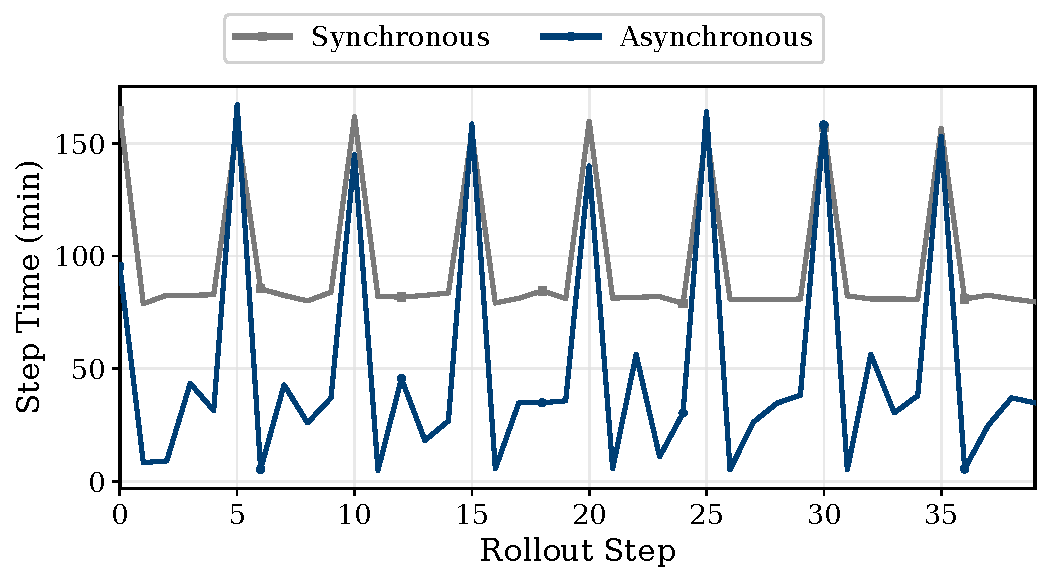
\includegraphics[width=0.55\linewidth]{figures/async_vs_sync_step_time.pdf}
  \caption{Wall-clock step-time comparison for synchronous and asynchronous rollout collection over 40 matched rollout steps. Mean step time is 97.0 minutes for the synchronous run and 50.8 minutes for the asynchronous run.}
  \label{fig:async-vs-sync-step-time}
\end{figure}

\subsection{Reward Normalization and Entropic Advantage}
\label{app:reward-advantage}

We distinguish three quantities: a score-derived \emph{base reward} used for logging and static comparisons, an adaptive-bound \emph{processed reward} used as the group reward when dynamic bounds are enabled, and an entropic processed advantage returned by the reward post-processing hook for RL updates.
For a raw task score $s$, define the signed score
\begin{equation}
\label{eq:signscore}
z =
\begin{cases}
s, & \text{if larger raw scores are better},\\
-s, & \text{otherwise}.
\end{cases}
\end{equation}
Static signed bounds are computed from task metadata after the same sign conversion. For larger-is-better metrics,
\begin{equation}
\label{eq:metric}
\begin{aligned}
B_{\mathrm{static}} &= \max(\texttt{theoretical\_max},\, \texttt{leaderboard\_max}), \\
W_{\mathrm{static}} &= \min(\texttt{theoretical\_min},\, \texttt{leaderboard\_min}),
\end{aligned}
\end{equation}
ignoring missing values; lower-is-better metrics use the corresponding signed versions of these quantities.

\textbf{Adaptive score range and processed reward.}
Fixed leaderboard or theoretical bounds can be much wider than the scores produced by the current policy, making two meaningfully different programs receive nearly the same reward. We instead rescale each task using a moving score range built from successful historical programs and the current rollout group. After converting every metric so that larger values are better, we sort the available scores as
\[
x_{(1)} \ge x_{(2)} \ge \cdots \ge x_{(K)} .
\]
The best observed score sets the upper end of the range. The 16th-best score sets the lower reference point; when fewer than 16 scores are available, we use the lowest available score:
\[
B_{\mathrm{dyn}} = x_{(1)},\qquad
W_{\mathrm{dyn}} = x_{(\min(16,K))}.
\]
We then extend the lower end downward by one quarter of the gap between these two reference scores. This keeps moderately successful programs from being clipped to zero when the observed scores are tightly clustered:
\[
W_{\mathrm{dyn}} \leftarrow W_{\mathrm{dyn}} - 0.25 \max(B_{\mathrm{dyn}}-W_{\mathrm{dyn}},0).
\]
When task metadata provides valid theoretical or leaderboard limits, they prevent the moving range from extending beyond the task's valid score range:
\[
B=\min(B_{\mathrm{dyn}},B_{\mathrm{static}}),\qquad
W=\max(W_{\mathrm{dyn}},W_{\mathrm{static}}),
\]
with fallback to static bounds if the resulting pair is invalid.
The resolved range maps scores to $[0,1]$ using the same transformation as Eq.~\ref{eq:base-reward}; scores below the lower end receive zero:
\[
r_{\mathrm{proc}}(z)=r_{\mathrm{base}}(z;B,W).
\]
Because the range is recomputed from recent and historical policy outputs, it follows the score frontier as training improves and preserves useful reward differences among current candidates. The implementation retains both static and adaptive reward views in metadata, while the adaptive view supplies the reward used by the main RL configuration.

\textbf{Entropic group advantages.}
This path replaces the usual GRPO-style normalization of group rewards into advantages.
When entropic post-processing is enabled, rewards are grouped by prompt group before advantage computation.
For group processed rewards $r_{\mathrm{proc},1},\ldots,r_{\mathrm{proc},K}$, the implementation returns zero advantages if $K<2$ or all rewards are equal.
Otherwise it centers rewards by $c_i=r_{\mathrm{proc},i}-\max_j r_{\mathrm{proc},j}$ and defines
\begin{equation}
\label{eq:entr}
q_i(\beta)=\frac{\exp(\beta c_i)}{\sum_{j=1}^{K}\exp(\beta c_j)}.
\end{equation}
The scalar $\beta$ is chosen by binary search so that
\begin{equation}
\label{eq:kl}
\mathrm{KL}\!\left(q_\beta\,\|\,\mathrm{Unif}(K)\right)
= \sum_{i=1}^{K} q_i(\beta)\left(\log q_i(\beta)+\log K\right)
\approx \log 2,
\end{equation}
with maximum search value $10^6$ and 60 bisection iterations.
The returned advantage for sample $i$ uses a leave-one-out denominator,
\[
e_i=\exp(\beta c_i),\qquad
Z_{-i}=\frac{1}{K-1}\sum_{j\ne i} e_j,\qquad
A_i=\frac{e_i}{Z_{-i}+10^{-12}}-1.
\]
The post-processing hook returns the input rewards as \texttt{raw\_rewards} and these $A_i$ values as \texttt{processed\_rewards}.


\subsection{Detection and prevention of reward hacking.}

During the training process, we observed that our models—particularly the smaller ones used in our early experiments—experience a specific issue during RL on difficult tasks. The reward quickly plateaus at a very low level.

Based on our case study, we discovered that the models are exhibiting significant reward hacking behavior. A representative example of this is when a model takes the sample submission, randomly shuffles it, and submits it as a solution.

To mitigate this, we implemented the following workflow:
1. We use o3-mini as an LLM judge during the RL process.
2. Before the code is executed in the sandbox, the judge performs a reward hack check.
3. If reward hacking is detected, the code bypasses sandbox execution and is assigned a reward of -0.5.

\section{\openmleevo{} Inference Details}

\subsection{Evolutionary Parent Fitness}
\label{app:evolutionary-fitness}

For a task $\tau$, let $\mathcal{P}_{\tau}$ be the set of programs stored in the task-local program database.
The implementation recomputes parent fitness at the task level after each insertion.
For each node $p\in\mathcal{P}_{\tau}$, define its linked children as
\[
\mathcal{C}(p)=\{c:\mathrm{parent}(c)=p\}\cup\{c:p\in \mathrm{crossover\_parents}(c)\}.
\]
The three raw components are:
\[
U_p = R^{\mathrm{base}}_p,
\]
\[
L_p =
\begin{cases}
\varnothing, & |\mathcal{C}(p)|=0,\\
0, & |\mathcal{C}(p)|=1,\\
\frac{1}{|\mathcal{C}(p)|}\sum_{c\in\mathcal{C}(p)}
\left(R^{\mathrm{base}}_c-\frac{1}{|\mathcal{C}(p)|}\sum_{c'\in\mathcal{C}(p)}R^{\mathrm{base}}_{c'}\right)^2,
& |\mathcal{C}(p)|\ge 2,
\end{cases}
\]
and
\[
V_p=|\mathcal{C}(p)|,\qquad
C^{\mathrm{raw}}_p =
\begin{cases}
1, & \max_{p'\in\mathcal{P}_{\tau}} V_{p'}=0,\\
\max\!\left(0,1-\frac{V_p}{\max_{p'\in\mathcal{P}_{\tau}}V_{p'}}\right), & \text{otherwise}.
\end{cases}
\]
For finite task-level values $\{a_p\}$, min--max normalization is
\[
N_{\eta}(a_p)=
\begin{cases}
\eta, & \max_{p'}a_{p'}-\min_{p'}a_{p'} < 10^{-12},\\
\frac{a_p-\min_{p'}a_{p'}}{\max_{p'}a_{p'}-\min_{p'}a_{p'}}, & \text{otherwise}.
\end{cases}
\]
The learning term uses optional normalization: missing $L_p=\varnothing$ receives the neutral value $\eta=0.5$, while finite learning values are normalized over only the finite entries.
Equivalently,
\[
N_{\eta}^{\mathrm{opt}}(L_p)=
\begin{cases}
\eta, & L_p=\varnothing,\\
N_{\eta}(L_p), & \text{otherwise, with } N_{\eta} \text{ computed over finite } \{L_{p'}\}.
\end{cases}
\]
The implemented fitness is
\[
F(p)=N_{0.5}(U_p)+N_{0.5}^{\mathrm{opt}}(L_p)+N_{0.5}(C^{\mathrm{raw}}_p).
\]
For \textsc{Improve} and \textsc{Crossover}, the candidate set is restricted to programs with positive stored reward; for \textsc{Debug}, it is restricted to programs with non-positive stored reward.
Within the candidate set $\mathcal{S}$, selection is roulette-wheel sampling without replacement:
\[
\Pr(p\mid \mathcal{S})=
\begin{cases}
\frac{\max(F(p),0)}{\sum_{p'\in\mathcal{S}}\max(F(p'),0)}, & \sum_{p'\in\mathcal{S}}\max(F(p'),0)>0,\\
\frac{1}{|\mathcal{S}|}, & \text{otherwise}.
\end{cases}
\]
Crossover draws two parents by applying this rule sequentially and removing the first sampled parent before the second draw.


\subsection{Operator Prompt Templates}
\label{app:openmleevo-operator-prompts}

\openmleevo{} uses four generation operators with distinct lineage context:
\textsc{Draft} proposes a new solution from the task specification,
\textsc{Improve} revises one selected parent, \textsc{Crossover} synthesizes two
selected parents, and \textsc{Debug} repairs a failed or non-positive-reward
parent. We reproduce below the complete system- and user-message schemas used
for MLE-Bench inference. Double-braced expressions denote task- or
attempt-specific runtime fields. To make the templates independent of a
particular search trajectory, optional retrieved memory and runtime data-preview
content are left empty; consequently, the empty-memory fallback text is shown.

\paragraph{\textsc{Draft}.}
\VerbatimInput[
  fontsize=\scriptsize,
  frame=single,
  framesep=1.5mm,
  framerule=0.3pt,
  rulecolor=\color{black!35},
  breaklines=true,
  breakanywhere=true,
  breaksymbolleft={}
]{sections/prompts/openmleevo_draft_prompt.txt}

\paragraph{\textsc{Improve}.}
\VerbatimInput[
  fontsize=\scriptsize,
  frame=single,
  framesep=1.5mm,
  framerule=0.3pt,
  rulecolor=\color{black!35},
  breaklines=true,
  breakanywhere=true,
  breaksymbolleft={}
]{sections/prompts/openmleevo_improve_prompt.txt}

\paragraph{\textsc{Crossover}.}
\VerbatimInput[
  fontsize=\scriptsize,
  frame=single,
  framesep=1.5mm,
  framerule=0.3pt,
  rulecolor=\color{black!35},
  breaklines=true,
  breakanywhere=true,
  breaksymbolleft={}
]{sections/prompts/openmleevo_crossover_prompt.txt}

\paragraph{\textsc{Debug}.}
\VerbatimInput[
  fontsize=\scriptsize,
  frame=single,
  framesep=1.5mm,
  framerule=0.3pt,
  rulecolor=\color{black!35},
  breaklines=true,
  breakanywhere=true,
  breaksymbolleft={}
]{sections/prompts/openmleevo_debug_prompt.txt}



\subsection{Structured Experience Records}
\label{app:openmleevo-experience-records}

\openmleevo{} represents inference-time search state with two deterministic structures. An \emph{experience card} is created after every sandbox evaluation and remains attached to that node. The task-level \emph{experience board} is recomputed from all accumulated cards whenever the controller needs global search state. Table~\ref{tab:openmleevo-experience-card-schema} gives the complete card content, and Table~\ref{tab:openmleevo-experience-board-schema} gives the board aggregation. We use \emph{experience board} consistently throughout the paper. The current evaluator persists the same object under the historical filename \nolinkurl{strategy_board.json} for backward compatibility; this filename does not denote a separate conceptual structure.

\begingroup
\small
\setlength{\tabcolsep}{5pt}
\renewcommand{\arraystretch}{1.12}
\setlength{\LTcapwidth}{\textwidth}
\begin{longtable}{@{}>{\raggedright\arraybackslash}p{0.17\textwidth}>{\raggedright\arraybackslash}p{0.39\textwidth}>{\raggedright\arraybackslash}p{0.38\textwidth}@{}}
\caption{Deterministic node-level experience-card schema in \openmleevo{}. The fields are populated from the program node, sandbox result, and usage record rather than inferred from test outcomes.}
\label{tab:openmleevo-experience-card-schema}\\
\toprule
\textbf{Card component} & \textbf{Stored fields} & \textbf{Role in search} \\
\midrule
\endfirsthead
\multicolumn{3}{c}{\tablename\ \thetable\ (continued)}\\
\toprule
\textbf{Card component} & \textbf{Stored fields} & \textbf{Role in search} \\
\midrule
\endhead
\midrule
\multicolumn{3}{r}{Continued on next page}\\
\endfoot
\bottomrule
\endlastfoot
Identity and lineage & \nolinkurl{schema_version}, \nolinkurl{node_id}, \nolinkurl{step_id}, \nolinkurl{operator}, \nolinkurl{parents}, \nolinkurl{parent_node_ids}, \nolinkurl{generation_id} & Identifies the evaluated program and reconstructs its incoming search edges. \\
Observed outcome & \nolinkurl{score}, \nolinkurl{fitness}, \nolinkurl{reward}, \nolinkurl{status}, \nolinkurl{status_code}, \nolinkurl{is_buggy}, \nolinkurl{error_signature} & Records the validation result and a normalized failure signature derived from execution status and logs. \\
Resource accounting & \nolinkurl{sandbox_time_used}, \nolinkurl{model_time_used}, \nolinkurl{model_plus_sandbox_time_used}, \nolinkurl{cost}, and prompt/completion/total token counts & Exposes the computational cost of the attempted method and supports budget-aware reasoning. \\
Method characterization & \nolinkurl{imports}, \nolinkurl{method_family_auto}, \nolinkurl{family_count_before} & Detects a coarse modeling family from the program and measures how often that direction has already been explored. \\
Derived search signals & \nolinkurl{delta_vs_parent}, \nolinkurl{novelty_score}, \nolinkurl{is_new_direction}, \nolinkurl{rank}, \nolinkurl{current_best}, \nolinkurl{selection_utility} & Supplies the progress and novelty factors used alongside validation quality, plus an auditable parent-selection trace. \\
Semantic evidence & \nolinkurl{plan}, \nolinkurl{analysis}, and optional \nolinkurl{rich_summary} with \nolinkurl{method_overview} and \nolinkurl{parent_comparison_experience} & Retains the model proposal and execution analysis; richer reusable summaries are generated lazily only when this node is retrieved. \\
\end{longtable}
\endgroup

\begingroup
\footnotesize
\setlength{\tabcolsep}{5pt}
\renewcommand{\arraystretch}{1.12}
\setlength{\LTcapwidth}{\textwidth}
\begin{longtable}{@{}>{\raggedright\arraybackslash}p{0.17\textwidth}>{\raggedright\arraybackslash}p{0.39\textwidth}>{\raggedright\arraybackslash}p{0.38\textwidth}@{}}
\caption{Task-global experience-board schema. The board is a deterministic aggregation of the cards available at the current search step.}
\label{tab:openmleevo-experience-board-schema}\\
\toprule
\textbf{Board component} & \textbf{Aggregated fields} & \textbf{Information exposed to the controller} \\
\midrule
\endfirsthead
\multicolumn{3}{c}{\tablename\ \thetable\ (continued)}\\
\toprule
\textbf{Board component} & \textbf{Aggregated fields} & \textbf{Information exposed to the controller} \\
\midrule
\endhead
\midrule
\multicolumn{3}{r}{Continued on next page}\\
\endfoot
\bottomrule
\endlastfoot
Global incumbent & \nolinkurl{num_nodes}, \nolinkurl{best_node}, \nolinkurl{best_score}, \nolinkurl{current_best_family} & The size and strongest valid member of the current population. \\
Method-family coverage & \nolinkurl{method_family_stats}, \nolinkurl{family_best_nodes}, \nolinkurl{underexplored_families} & Per-family counts, valid/failure counts, best score and node, failure rate, and low-coverage directions. \\
Progress and failures & \nolinkurl{score_history}, \nolinkurl{recent_delta_trend}, \nolinkurl{repeated_errors}, \nolinkurl{status_count}, \nolinkurl{operator_counts} & Recent search progress, recurring error signatures, and the empirical mix of operators and outcomes. \\
Topology and node state & \nolinkurl{parent_graph}, \nolinkurl{novelty_by_node}, \nolinkurl{rank_by_node}, \nolinkurl{current_best_by_node} & Reconstructs ancestry and provides per-node novelty, rank, and incumbent indicators for retrieval. \\
Resources and audit trail & \nolinkurl{runtime_stats}, \nolinkurl{parent_selection_weights} & Aggregates model/sandbox runtime and preserves the candidate factors, utilities, probabilities, and selected IDs from parent sampling. \\
\end{longtable}
\endgroup

\paragraph{Grounded record.}
For a successful \textsc{Improve} node on \texttt{leaf-classification}, the stored card records \nolinkurl{step_id=10}, validation log loss \nolinkurl{fitness=0.012080}, \nolinkurl{delta_vs_parent=0.753352}, \nolinkurl{method_family_auto=ensemble+xgboost+neural_net+cv}, \nolinkurl{novelty_score=0.57735}, \nolinkurl{rank=1}, \nolinkurl{current_best=true}, 178.58 seconds of sandbox time, and 24,564 total model tokens. Immediately before generating this node, the experience board identified a \nolinkurl{neural_net+cv} incumbent with score 0.031825, reported three previous timeouts, and exposed a recent mean parent-relative gain of 0.01649. Thus, the card states exactly what the new node achieved, while the board states where that result sits within the surrounding population.

\subsection{Experience-Guided Parent Selection}
\label{app:openmleevo-parent-selection}

This subsection specifies the inference-time parent-selection rule used by \openmleevo{} and is distinct from the training-time parent fitness in Appendix~\ref{app:evolutionary-fitness}. For a sampled island $\mathcal{I}$, each candidate $i\in\mathcal{I}$ is associated with a deterministic experience card. Let $s_i$ denote its validation score and let $s_i^{\mathrm{par}}$ be the score of its strongest parent under the task metric. The default score component applies direction-aware min--max normalization:
\[
\tilde{s}_i =
\begin{cases}
\dfrac{s_i-s_{\min}}{s_{\max}-s_{\min}}, & \text{if higher is better},\\[6pt]
\dfrac{s_{\max}-s_i}{s_{\max}-s_{\min}}, & \text{if lower is better}.
\end{cases}
\]
When all candidate scores are equal, we set $\tilde{s}_i=0.5$. The improvement component retains only progress over the best available parent:
\[
\Delta_i =
\begin{cases}
\max(0,s_i-s_i^{\mathrm{par}}), & \text{if higher is better},\\
\max(0,s_i^{\mathrm{par}}-s_i), & \text{if lower is better},
\end{cases}
\qquad
\widetilde{\Delta}_i =
\begin{cases}
\dfrac{\Delta_i}{\max_{j\in\mathcal{I}}\Delta_j}, & \max_{j\in\mathcal{I}}\Delta_j>0,\\[6pt]
0, & \text{otherwise}.
\end{cases}
\]
Nodes without a valid parent receive zero improvement. Finally, if $N_{f_i}$ is the number of other previously recorded cards in candidate $i$'s automatically detected method family $f_i$, the novelty component is
\[
\nu_i = \frac{1}{\sqrt{1+N_{f_i}}}.
\]
The utility and temperature-controlled softmax are given in Equation~\ref{eq:openmleevo-parent-selection}. The default implementation uses min--max normalization for score and improvement, while rank-based and hybrid normalizations are configurable. For \textsc{Crossover}, two parents are sampled sequentially without replacement from the same island; for \textsc{Improve}, one parent is sampled. Final submission selection is not sampled: it deterministically chooses the best executable candidate with a valid validation outcome.

\thispagestyle{fancy}

\subsection{Operation-Triggered Memory Synthesis}
\label{app:openmleevo-memory-synthesis}

The controller stores every deterministic experience card, but it does not eagerly ask a language model to summarize every node. Once an operation and its parent nodes have been selected, it first retrieves a bounded, operation-specific evidence set (Table~\ref{tab:openmleevo-operation-memory}). For any retrieved node without a cached rich summary, the memory model receives the task description; current and parent metadata; both plans, programs, and execution outputs; score, parent-relative delta, runtime, status, and error signature. It must return exactly two JSON fields: \nolinkurl{method_overview}, a concrete description of the model, features, validation, ensembling, runtime choices, and submission logic; and \nolinkurl{parent_comparison_experience}, an evidence-based account of what changed, whether score/status/runtime improved, and what should be reused or avoided. Each synthesis call summarizes one retrieved node relative to one direct parent; when an operation retrieves multiple nodes or two crossover branches, their independently cached summaries are composed only in the subsequent operator-specific context. The resulting summary is cached in the node and its card, so later operations reuse it without another synthesis call. 

\begingroup
\footnotesize
\setlength{\tabcolsep}{5pt}
\renewcommand{\arraystretch}{1.12}
\begin{longtable}{@{}>{\raggedright\arraybackslash}p{0.13\textwidth}>{\raggedright\arraybackslash}p{0.46\textwidth}>{\raggedright\arraybackslash}p{0.35\textwidth}@{}}
\caption{Operation-conditioned memory retrieval in \openmleevo{}. Ancestor, sibling, and related-node caps are configurable; the table reports the defaults used by the implementation.}
\label{tab:openmleevo-operation-memory}\\
\toprule
\textbf{Operator} & \textbf{Default retrieved evidence} & \textbf{Purpose of the rendered memory} \\
\midrule
\endfirsthead
\multicolumn{3}{c}{\tablename\ \thetable\ (continued)}\\
\toprule
\textbf{Operator} & \textbf{Default retrieved evidence} & \textbf{Purpose of the rendered memory} \\
\midrule
\endhead
\midrule
\multicolumn{3}{r}{Continued on next page}\\
\endfoot
\bottomrule
\endlastfoot
\textsc{Draft} & No inherited node memory. & Starts an independent branch from the task specification. \\
\textsc{Improve} & The selected parent, its three most recent ancestors, and its top three direct siblings. Siblings share at least one parent and are ranked by the same quality--progress--novelty utility used for parent selection. Relevant board fields are appended. & Preserves what works in the parent, identifies changes that helped or hurt along its lineage, and contrasts nearby alternatives without replaying the full tree. \\
\textsc{Crossover} & Two selected parents; for each parent, two recent ancestors and two top-ranked direct siblings; family-level statistics, repeated errors, and a method-family complementarity cue. & Identifies compatible strengths and conflicts between branches and discourages a mechanical concatenation of both programs. \\
\textsc{Debug} & The current buggy node followed first by prior nodes with the same error signature and then by recent attempts, up to a default total of three related nodes; repeated-error counts are included. & Reuses fixes for the same failure mode while retaining a recent-context fallback for previously unseen errors. \\
\end{longtable}
\endgroup

The rendered memory groups selected cards, cached summaries, and board fields into named sections. \textsc{Improve} receives the selected parent, vertical ancestors, horizontal siblings, and related board statistics; \textsc{Crossover} repeats the branch sections for both parents and adds the complementarity cue; and \textsc{Debug} receives the current signature, repeated-error counts, current buggy node, and related errors. This bounded branch-local context replaces an unbounded concatenation of prior analyses. The exact system and user-message templates are provided below.

\hypertarget{openmleevo-rich-memory-prompt}{\paragraph{Complete rich-memory synthesis prompt.}}
The production system prompt and parameterized user-message template used to extract reusable memories from past trajectories are shown below. Double-braced expressions denote runtime fields populated from the task, the current node, and its direct parent.


\VerbatimInput[
  fontsize=\scriptsize,
  frame=single,
  framesep=1.5mm,
  framerule=0.3pt,
  rulecolor=\color{black!35},
  breaklines=true,
  breakanywhere=true,
  breaksymbolleft={}
]{sections/prompts/openmleevo_rich_memory_summary_prompt.txt}

\paragraph{Grounded rendered context.}
In the \texttt{leaf-classification} example, the selected ResNet50, handcrafted-geometry, and XGBoost parent had log loss 0.765432. Horizontal memories exposed a simpler ResNet18 plus tabular-feature incumbent at 0.031825 and a feature-heavy sibling that timed out after 7,200 seconds; the board reported \nolinkurl{current_best_family=neural_net+cv}, \nolinkurl{repeated_errors: timeout=3}, and the parent-family best and failure rate. The next \textsc{Improve} operation accordingly dropped the oversized ResNet50 and slow handcrafted pipeline, retained ResNet18 and tabular features, and added calibrated out-of-fold ensembling, yielding 0.012080. This grounds generated memory in both local alternatives and global search state.

\section{Supplementary Experiments}

\subsection{Repeated-Evaluation Statistics on MLE-Bench Lite}
\label{app:openmle-repeat-evaluation}

For model--harness configurations with available repeat-level records, we
aggregate three evaluation epochs and report the corresponding mean and
standard deviation in Table~\ref{tab:openmle-repeat-results}. Repeated
evaluation reduces sensitivity to favorable sampling trajectories and
transient sandbox behavior, while the standard deviation quantifies the
remaining run-to-run variability.

Owing to the substantial inference and sandbox cost, Codex, Claude Code,
and Gemini CLI references were evaluated only once and are
therefore retained as point estimates in the main results table. Entries
without $\pm$ in Table~\ref{tab:openmle-repeat-results} indicate metrics
for which the archived summary contains the aggregate estimate but not
the underlying repeat-level dispersion. All reported $\pm$ values denote
standard deviations rather than confidence intervals.

\begin{table*}[t]
\centering
\scriptsize
\setlength{\tabcolsep}{5.5pt}
\renewcommand{\arraystretch}{1.10}
\caption{
Repeated-evaluation results on MLE-Bench Lite under the OpenMLE
harnesses. Values are mean $\pm$ standard deviation across three
evaluation epochs. Valid Rate is the mean number of tasks producing
valid submissions out of 22; Medal Average and Human Rank are
higher-is-better. 
}
\label{tab:openmle-repeat-results}
\begin{tabular}{@{}llccc@{}}
\toprule
Model / system
& Framework
& Valid Rate
& Medal Average $\uparrow$
& Human Rank $\uparrow$ \\
\midrule

\shortstack[l]{Qwen3-30B-A3B-Thinking-2507}
& \openmleevo{}
& $17.33 \pm 0.47$/22
& $34.85\% \pm 2.14\%$
& $0.5573 \pm 0.0074$ \\

Frontis-MA1-30B
& \openmleevo{}
& $21.67 \pm 0.47$/22
& $53.03\% \pm 4.29\%$
& $0.7055 \pm 0.0505$ \\

Frontis-MA1-30B
& \openmleevomax{}
& $22.00 \pm 0.00$/22
& $66.67\% \pm 5.67\%$
& $0.8053 \pm 0.0236$ \\

\addlinespace[2pt]

Qwen3.6-35B-A3B
& \openmleevo{}
& $19.67 \pm 0.47$/22
& $39.39\% \pm 5.67\%$
& $0.5828 \pm 0.0278$ \\

Frontis-MA1-35B
& \openmleevo{}
& $21.67 \pm 0.47$/22
& $60.61\% \pm 7.73\%$
& $0.7647 \pm 0.0376$ \\

Frontis-MA1-35B
& \openmleevomax{}
& $22.00 \pm 0.00$/22
& $\mathbf{71.21\% \pm 8.57\%}$
& $0.8126 \pm 0.0388$ \\
\midrule

GLM-5.2
& \openmleevomax{}
& $22.00 \pm 0.00$/22
& $66.67\% \pm 8.57\%$
& $\mathbf{0.8164 \pm 0.0233}$ \\

MiniMax M3
& \openmleevo{}
& $22.00 \pm 0.00$/22
& $59.09\% \pm 0.00\%$
& $0.7994 \pm 0.0225$ \\

MiniMax M3
& \openmleevomax{}
& $22.00 \pm 0.00$/22
& $65.15\% \pm 2.14\%$
& $0.8007 \pm 0.0089$ \\

Kimi K2.6
& \openmleevo{}
& $21.67 \pm 0.47$/22
& $66.67\% \pm 5.67\%$
& $0.7859 \pm 0.0285$ \\

Grok-4.5
& \openmleevo{}
& $22.00 \pm 0.00$/22
& $65.15\% \pm 2.14\%$
& $0.8052 \pm 0.0170$ \\

LongCat-2.0
& \openmleevo{}
& $21.00 \pm 0.82$/22
& $56.06\% \pm 5.67\%$
& $0.7343 \pm 0.0150$ \\

Doubao Seed 2.1 Pro
& \openmleevo{}
& $20.33 \pm 0.47$/22
& $56.06\% \pm 2.14\%$
& $0.7170 \pm 0.0397$ \\

Qwen3.7 Plus
& \openmleevo{}
& $21.67 \pm 0.47$/22
& $54.55\% \pm 6.43\%$
& $0.7234 \pm 0.0408$ \\

DeepSeek-V4-Pro
& \openmleevo{}
& $21.67 \pm 0.47$/22
& $54.55\% \pm 3.71\%$
& $0.6849 \pm 0.0258$ \\

DeepSeek-V4-Flash
& \openmleevo{}
& $21.33 \pm 0.47$/22
& $51.52\% \pm 5.67\%$
& $0.6957 \pm 0.0200$ \\

GLM-4.7
& \openmleevo{}
& $21.33 \pm 0.47$/22
& $51.52\% \pm 7.73\%$
& $0.6521 \pm 0.0543$ \\

MiniMax M2.7
& \openmleevo{}
& $22.00 \pm 0.00$/22
& $50.00\% \pm 7.42\%$
& $0.7039 \pm 0.0298$ \\

MiMo-V2.5-Pro
& \openmleevo{}
& $17.00 \pm 1.63$/22
& $40.91\% \pm 3.71\%$
& $0.5213 \pm 0.0422$ \\

Step-3.7 Flash
& \openmleevo{}
& $19.00 \pm 0.00$/22
& $27.27\% \pm 6.43\%$
& $0.4953 \pm 0.0385$ \\

\bottomrule
\end{tabular}
\end{table*}

\subsection{NatureBench Lite Task Composition}
\label{app:naturebench-lite}

Our generalization study uses the fixed 10-task NatureBench Lite subset summarized in Table~\ref{tab:naturebench-lite-tasks}.
The subset favors moderately tractable tasks while preserving coverage across all six NatureBench scientific domains and diverse data structures, including biological sequences, omics matrices, molecular structures, temporal signals, images, and tabular features.
This breadth makes the subset useful for rapid model--harness comparisons, but its ten-task size means that each task changes All S or All M by ten percentage points.

\section{Simplified comparison of public release surfaces}

The public release landscape remains fragmented. Table~\ref{tab:mle-open-release-matrix} summarizes representative MLE-agent and MLE-resource work by the artifacts needed to reproduce a full post-training stack. Scores are not strictly comparable because the systems differ in backbone
model, compute and wall-clock budgets, hardware, external-resource access,
number of runs, and aggregation procedure. Checkmarks denote artifacts that
were publicly accessible and independently verifiable from the cited paper or
repository at the time of audit. High-scoring systems often release an inference framework, evaluation entry point, or leaderboard result; resource projects provide tasks and environments; training-oriented papers describe RL designs for MLE agents~\citep{qiang2025mlesmith,liu2025mlagent,li2025mlerl,yang2025rlmleagents,cai2026acegrpo}. Across these threads, the combination of executable training data, sandbox infrastructure, training code, RL method, evaluation framework, and model weights is still rare. This gap motivates treating open MLE capability as a full-stack problem spanning data, execution, optimization, and inference.

\begin{table}[htbp]
\centering
\caption{The 10 tasks in NatureBench Lite used for the generalization experiment.}
\label{tab:naturebench-lite-tasks}
\vspace{0.4em}
\scriptsize
\setlength{\tabcolsep}{3pt}
\renewcommand{\arraystretch}{1.1}
\begin{tabular}{@{}>{\raggedright\arraybackslash}p{0.31\linewidth}>{\raggedright\arraybackslash}p{0.17\linewidth}>{\raggedright\arraybackslash}p{0.24\linewidth}>{\raggedright\arraybackslash}p{0.20\linewidth}@{}}
\toprule
Task & Domain & Input modality & ML task type \\
\midrule
Spatial RNA Velocity Inference & Cellular Omics & Single-cell and spatial omics & Simulation / operator learning \\
Disease-Specific Variant Effect Prediction & Cellular Omics & Biological sequence & Prediction / regression \\
Metabolomic Profile Prediction from Microbial Composition & Cellular Omics & Tabular / feature matrix & Prediction / regression \\
Protein Variant Effect Prediction & Protein Biology & Biological sequence & Prediction / regression \\
Lasso Peptide Property Prediction & Protein Biology & Biological sequence & Prediction / regression \\
Anomalous Diffusion Out-of-Distribution Dynamics Detection & Physical Modeling & Temporal / signal / spectra & Classification \\
Zeolite--Molecule Binding Affinity Prediction & Physical Modeling & Molecular / materials structure & Prediction / regression \\
Spatial Clustering of Single-Molecule Localization Point Clouds & Biomedical Modeling & Image / volumetric & Clustering / integration \\
Molecular Property Prediction & Molecular Design & Molecular / materials structure & Prediction / regression \\
Categorical Counterfactual Outcome Estimation & Relational Reasoning & Tabular / feature matrix & Classification \\
\bottomrule
\end{tabular}
\end{table}


\begin{table}[H]
\centering
\caption{
Audited comparison of public release surfaces for representative MLE agents and resources.
Artifact availability was rechecked against the cited papers, official repositories, and the official MLE-Bench leaderboard submissions as of July 2026.
}
\label{tab:mle-open-release-matrix}
\vspace{0.3em}
\scriptsize
\setlength{\tabcolsep}{2.6pt}
\renewcommand{\arraystretch}{1.08}
\resizebox{\linewidth}{!}{%
\begin{tabular}{@{}lccccccccc@{}}
\toprule
Work
& Data
& Sandbox
& \shortstack{Train\\code}
& \shortstack{RL\\method}
& Eval
& Weights
& \shortstack{MLE-Bench Lite\\Medal Rate}
& \shortstack{Run\\setting}
& Best model \\
\midrule

\multicolumn{10}{@{}l}{\textit{No trained MLE model released}} \\

AIDE~\citep{jiang2025aide}
& \xmark & \cmark & \xmark & \xmark & \cmark & \xmark
& 35.91\%
& \mbox{24h $\cdot$ 1$\times$A10}
& o1-preview \\

AutoMLGen / InternAgent~\citep{du2025automlgen}
& \xmark & \cmark & \xmark & \xmark & \cmark & \xmark
& 62.12\%
& \mbox{12h $\cdot$ 1$\times$A800}
& DeepSeek-R1 \\

ML-Master 2.0~\citep{liu2025ml,zhu2026toward}
& \xmark & \cmark & \xmark & \xmark & \cmark & \xmark
& 75.76\%
& \mbox{24h $\cdot$ 2$\times$RTX~4090}
& DeepSeek-V3.2-Speciale \\

MLE-STAR-Pro-1.5~\citep{nam2025mlestar}
& \xmark & \cmark & \xmark & \xmark & \cmark & \xmark
& 68.18\%
& \mbox{24h $\cdot$ 2$\times$A100-40G}
& Gemini-2.5-Pro \\

MLZero~\citep{fang2025mlzero}
& \xmark & \cmark & \xmark & \xmark & \cmark & \xmark
& 36.36\%$^{\dagger}$
& \mbox{24h $\cdot$ 8$\times$A100-40G}
& Claude-Sonnet-3.7 \\

AIRA-dojo~\citep{toledo2025airesearchagents}
& \xmark & \cmark & \xmark & \xmark & \cmark & \xmark
& 55.00\%
& \mbox{24h $\cdot$ 1$\times$H200}
& o3 \\

Famou-Agent 2.0~\citep{li2025fmagent}
& \xmark & \xmark & \xmark & \xmark & \cmark & \xmark
& 80.30\%
& \mbox{24h $\cdot$ 1$\times$A800}
& Gemini-3-Pro-Preview \\

MLEvolve~\citep{du2026mlevolve}
& \xmark & \cmark & \xmark & \xmark & \cmark & \xmark
& 80.30\%
& \mbox{12h $\cdot$ 1$\times$H200}
& Gemini-3-Pro-Preview \\

AIBuildAI~\citep{zhang2026aibuildai}
& \cmark & \cmark & \xmark & \xmark & \cmark & \xmark
& 77.27\%
& \mbox{24h $\cdot$ 1$\times$A100}
& Claude-Opus-4.6 \\

MLAgentBench~\citep{huang2023mlagentbench}
& \cmark & \cmark & \xmark & \xmark & \cmark & \xmark
& --
& --
& -- \\

MLGym~\citep{nathani2025mlgym}
& \cmark & \cmark & \xmark & \xmark & \cmark & \xmark
& --
& --
& -- \\

MLE-Dojo~\citep{qiang2025mledojo}
& \cmark & \cmark & \xmark & \xmark & \cmark & \xmark
& --
& --
& -- \\

MLE-Smith~\citep{qiang2025mlesmith}
& \xmark & \xmark & \xmark & \xmark & \xmark & \xmark
& --
& --
& -- \\

R\&D-Agent~\citep{yang2025r}
& \xmark & \cmark & \xmark & \xmark & \cmark & \xmark
& 68.18\%
& \mbox{12h $\cdot$ 1$\times$V100}
& GPT-5 \\

\midrule
\multicolumn{10}{@{}l}{\textit{Post-trained MLE agents}} \\

RL-MLE~\citep{yang2025rlmleagents}
& \xmark & \xmark & \xmark & \cmark & \xmark & \xmark
& --
& --
& -- \\

ML-Agent~\citep{liu2025mlagent}
& \xmark & \xmark & \cmark$^{\ddagger}$ & \cmark & \xmark & \xmark
& --
& --
& -- \\

MLE-RL~\citep{li2025mlerl}
& \xmark & \xmark & \xmark & \cmark & \xmark & \xmark
& 33.30\%
& \mbox{12h $\cdot$ A10 (count NR)}
& MLE-RL-32B-S \\

AceGRPO~\citep{cai2026acegrpo}
& \xmark & \xmark & \xmark & \cmark & \xmark & \xmark
& 51.52\%
& \mbox{12h $\cdot$ GPU NR}
& Ace-30B \\

\textbf{OpenMLE (ours)}
& \cmark & \cmark & \cmark & \cmark & \cmark & \cmark
& \textbf{\frontisThirtyFiveEvoMaxResult{}}
& \mbox{12h $\cdot$ RTX~4090(12G VRAM)}
& \thirtyfivebmodel{} \\

\bottomrule
\end{tabular}%
}

\vspace{0.3em}
\begin{minipage}{\linewidth}
\tiny
\textit{Release criteria.}
For \emph{Data}, \emph{Sandbox}, \emph{Train code}, \emph{Eval}, and
\emph{Weights}, a tick requires an artifact that was publicly accessible
at the time of audit.
\emph{Data} requires downloadable task/training data or scripts for
reconstructing it; \emph{Sandbox} requires released code capable of
running model-generated programs or constructing their execution
environment; \emph{Train code} requires model-parameter training
entry points or configurations; \emph{Eval} accepts runnable evaluation
assets or official per-run grading reports; and \emph{Weights} requires
downloadable trained MLE-agent weights.
A tick under \emph{RL method} indicates that the work develops or applies
an MLE-specific RL post-training method; it does not by itself imply that
the RL implementation is public.
Run settings report the per-task wall-clock limit and sandbox GPU
allocation; remote LLM-serving compute and CPU/RAM are omitted.
NR means not reported, and ``--'' means that no corresponding
MLE-Bench Lite result is available.
GPU-h denotes total sandbox accelerator time rather than elapsed
wall-clock time.

$^{\dagger}$ MLZero evaluated 21 of the 22 MLE-Bench Lite tasks,
excluding one task because of preprocessing inconsistencies.
The displayed rate uses the standard 22-task denominator, counting
the excluded task as a non-medal result.

$^{\ddagger}$ ML-Agent currently releases its exploration-enriched SFT
training code only; its step-wise RL implementation, training dataset,
evaluation code, and model checkpoints remain unreleased.
\end{minipage}
\end{table}
